\subsection{Task 1.1.1: Polynomial Basis Functions}

\subsubsection{Aufgabenstellung:}


Es sollen die Gewichtungsfaktoren für Polynome vom 0ten Grad bis zum 18ten Grad gefunden werden, dazu sind die 60 gegebenen X- und Y-Trainingswerte zu verwenden.


Danach sind die Trainingspunkte, die Target-Funktion(y\_target) und die ``Lern-funktionen'' zu Auszugeben.


Die Basisfunktionen als Funktion von X ausgeben.

Ausgeben des ``Mean Squared Error'' (MSE) für die Trainings- und Test- werte.


\subsubsection{Plots \& Diskussion:}
\begin{figure}[hp!]
\begin{center}
 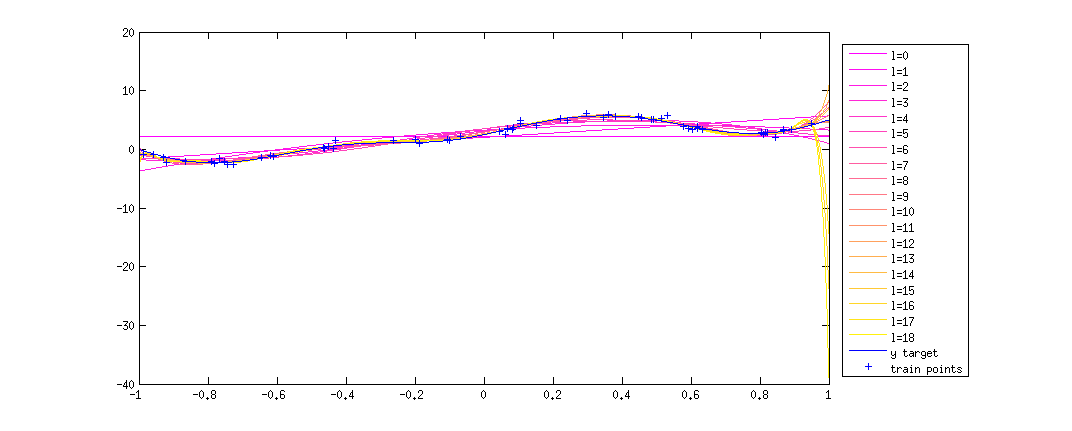
\includegraphics[width=0.99\textwidth]{./figures/1_1_1_unscaled_learn_fct}
 \caption[Unskalierte Lernfunktionen]{Unskalierte Lernfunktionen}
\label{fig:unscaled_learn_fct}
\end{center}
\end{figure}


\begin{figure}[hp!]
\begin{center}
 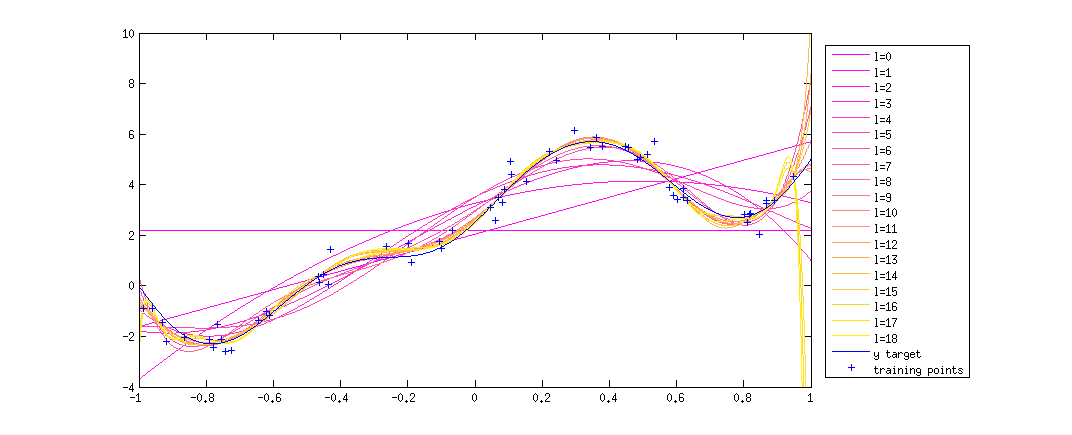
\includegraphics[width=1\textwidth]{./figures/1_1_1_scal_learn_fct}
 \caption[Skalierte Lernfunktionen]{Skalierte Lernfunktionen}
\label{fig:scal_learn_fct}
\end{center}
\end{figure}

In Abbildung \ref{fig:unscaled_learn_fct} sehen wir die Lernfunktionen.
In Abb. \ref{fig:unscaled_learn_fct} reisen die Werte für Polynome höheren Grades am Ende des ``Plots'' sehr stark aus.
 Das Bild wird somit in Y-Richtung gequetscht wird, in Abb. \ref{fig:scal_learn_fct} das ganze noch einmal skaliert um mehr zu erkennen.

\begin{figure}[hp!]
\begin{center}
 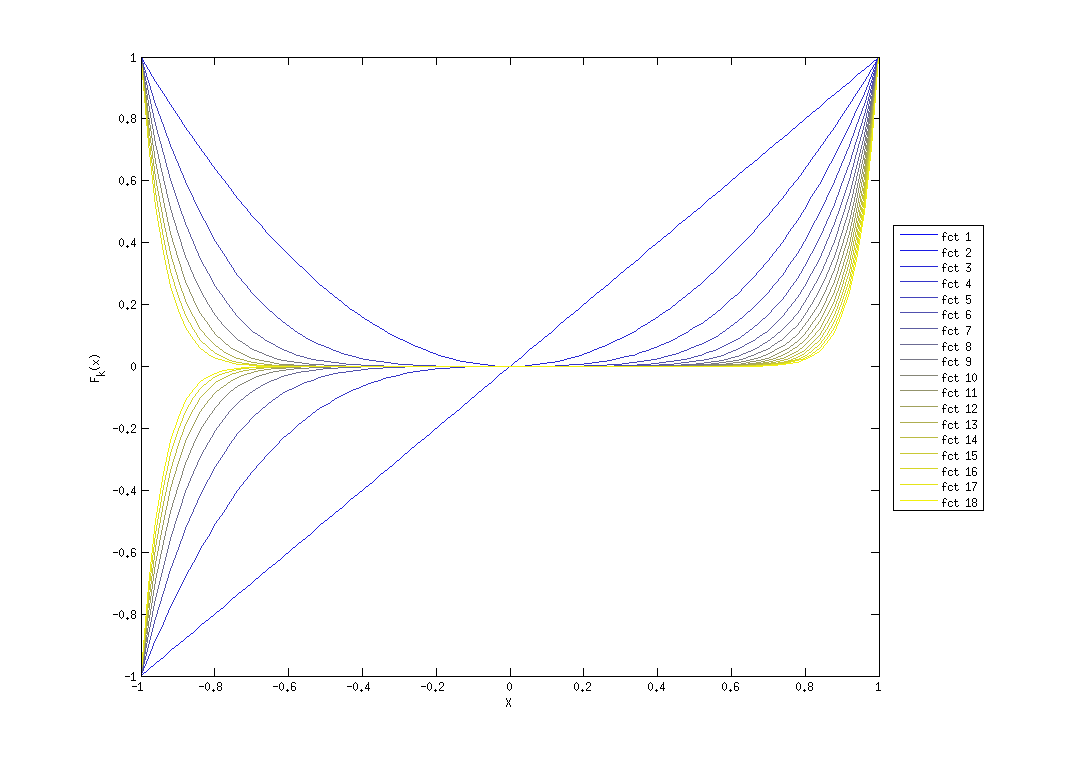
\includegraphics[width=1\textwidth]{./figures/1_1_1_base_fct}
 \caption[Basisfunktionen als Funktion von X]{Basisfunktionen als Funktion von X}
\label{fig:base_fct}
\end{center}
\end{figure}
In Abb. \ref{fig:base_fct} kann man Sehen das Funktionen höherer Ordnung sehr stark einknicken. Das bedeutet das sich Funktionen höherer Ordnung 
schneller bzw. stärker den Testdaten anpassen. Allerdings sollt hier ein Mittel gefunden werden, da die Testdaten ja auch nicht exakt und mit
Rauschen behaftet sind! 



Bei Funktionen mit höheren Polynomen ist die Funktion zwar sehr gut eingepasst an die Trainingspunkte, neigt aber zu starkem Überschwingen.
Das sog. ``Overfitting'' tritt hier auf.
\clearpage

\begin{figure}[hp!]
\begin{center}
 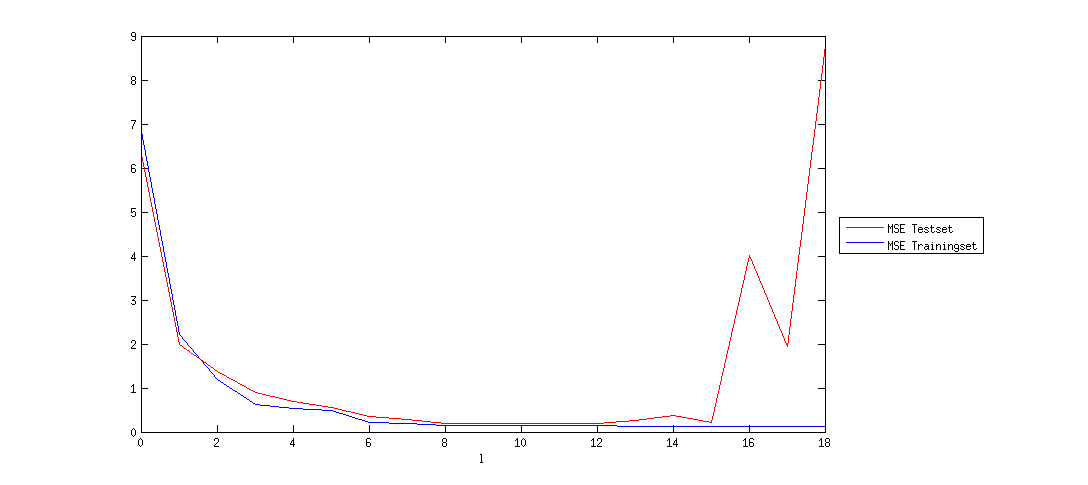
\includegraphics[width=1\textwidth]{./figures/1_1_1_MSE}
 \caption[Mean Square Error]{Mean Square Error für Trainings- und Test-Werte}
\label{fig:MSE}
\end{center}
\end{figure}

Wie man in Abb. \ref{fig:MSE} sehen kann ist bereits bei einer Funktion mit Grad 8 der Fehler sehr gering,bei Grad 8 ist  
Aufwand und Leistung am Besten. Es ist die Funktion nur für die Trainings-Werte 
perfekt angepasst allerdings wird durch das ``OverFitting'' für alle anderen Werte der Fehler wieder größer.